
\definecolor{high}{RGB}{76, 175, 80}    % Зеленый
\definecolor{medium}{RGB}{255, 193, 7}  % Желтый
\definecolor{low}{RGB}{244, 67, 54}     % Красный

Аналогично, будем использовать \textbf{логистическую регрессию}\\

\hspace*{-1cm}
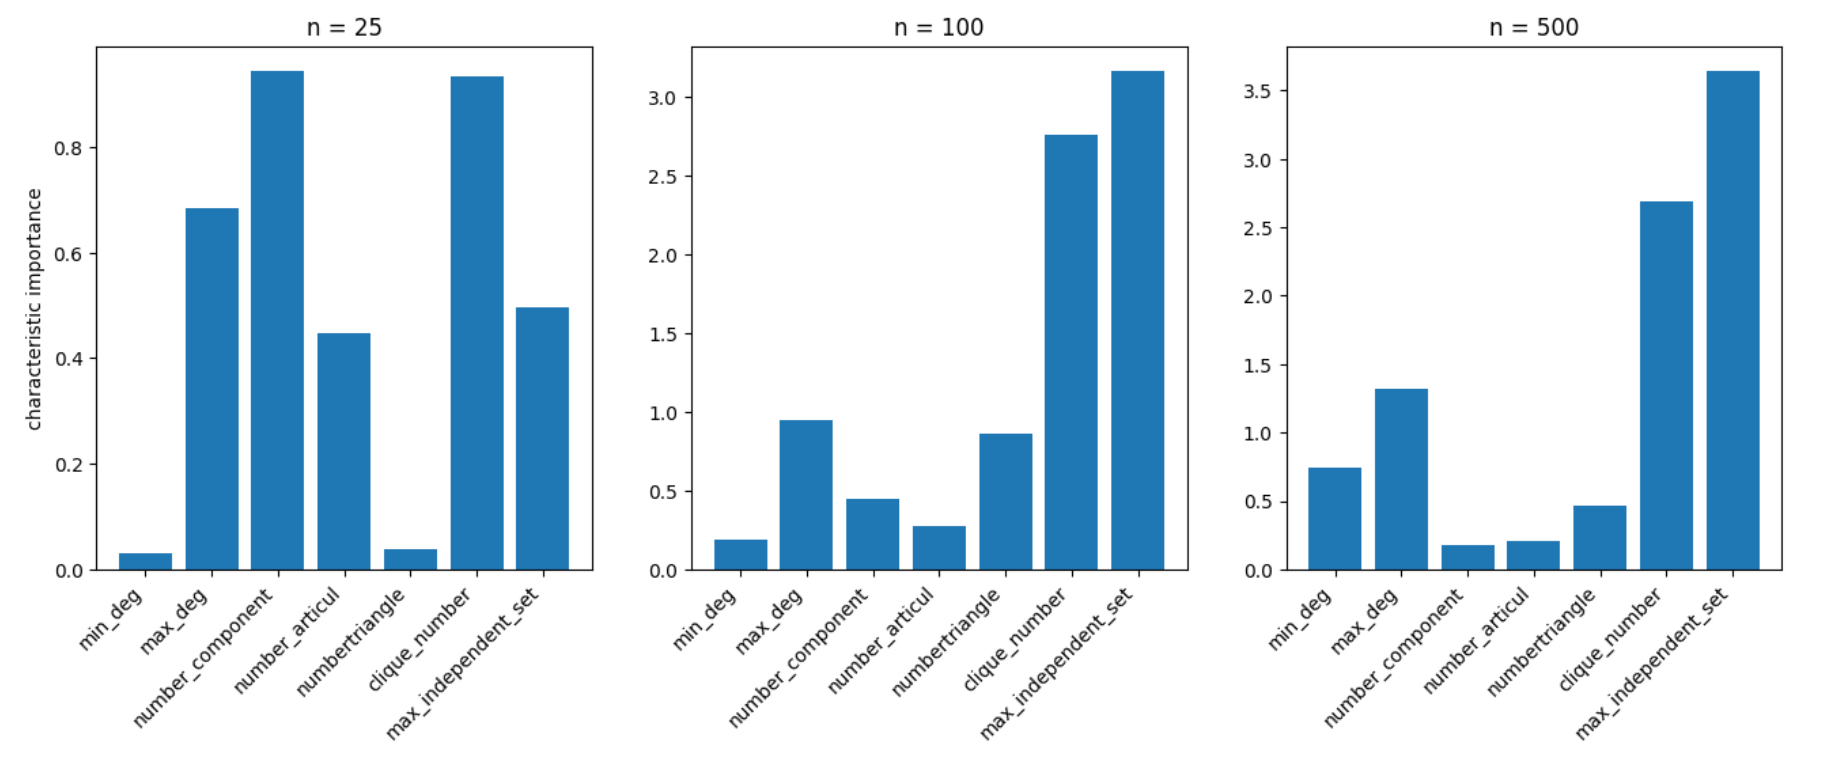
\includegraphics[width=1\textwidth]{Part-II-Ivanova/stats.png}\\ 

\textbf{Вывод:} \\

\begin{table}[h]
    \centering
    \begin{minipage}{0.7\textwidth}
    \centering
    \scalebox{0.8}{
    \begin{tabular}{|>{\raggedright}p{4cm}|c|c|c|}
    \hline
    \textbf{Характеристика графа} & \textbf{n=25} & \textbf{n=100} & \textbf{n=500} \\ 
    \hline
    Минимальная степень   & \cellcolor{low} & \cellcolor{low} & \cellcolor{medium} \\ 
    \hline 
    Максимальная степень & \cellcolor{high} & \cellcolor{medium} & \cellcolor{medium} \\
    \hline
    Количество компонент связности & \cellcolor{high} & \cellcolor{medium} & \cellcolor{low} \\
    \hline
    Количество точек сочленения & \cellcolor{medium} & \cellcolor{low} & \cellcolor{low} \\
    \hline
    Количество треугольников & \cellcolor{low} & \cellcolor{medium} & \cellcolor{low} \\
    \hline
    Кликовое число графа & \cellcolor{high} & \cellcolor{high} & \cellcolor{high} \\
    \hline
    Число независимости & \cellcolor{medium} & \cellcolor{high} & \cellcolor{high} \\
    \hline
    \end{tabular}
    }
    \label{tab:importance}
    \end{minipage}%
    \begin{minipage}{0.3\textwidth}
    \centering
    \begin{tabular}{ll}
    \cellcolor{high} & Высокая важность \\
    \cellcolor{medium} & Средняя важность \\
    \cellcolor{low} & Низкая важность \\
    \end{tabular}
    \end{minipage}
\end{table}
\\


